\tikzset{every picture/.style={line width=0.75pt}}
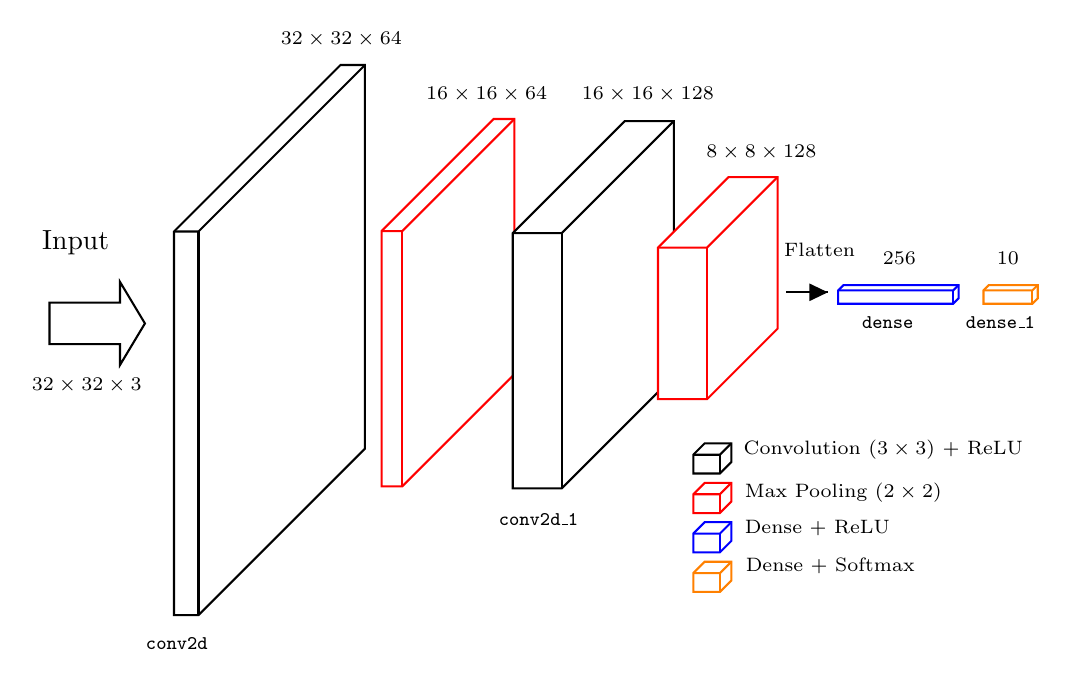
\begin{tikzpicture}[x=0.75pt,y=0.75pt,yscale=-1,xscale=1]

% --- MODEL BLOCKS ---

% Input
\draw   (-10,140) -- (24,140) -- (24,130) -- (36,150) -- (24,170) -- (24,160) -- (-10,160) -- cycle ;
\draw (-15,104) node [anchor=north west][inner sep=0.75pt]   [align=left] {Input};
\draw (-20,175) node [anchor=north west][inner sep=0.75pt]  [font=\scriptsize]  {$32\times 32\times 3$};

% Conv1 (64)
\draw  [fill=white  ,fill opacity=1 ] (50, 105.69) -- (130.19, 25.5) -- (142, 25.5) -- (142, 210.31) -- (61.81, 290.5) -- (50, 290.5) -- cycle ;
\draw   (142, 25.5) -- (61.81, 105.69) -- (50, 105.69) ; \draw   (61.81, 105.69) -- (61.81, 290.5) ;
\draw (100, 8) node [anchor=north west][inner sep=0.75pt]  [font=\scriptsize] {$32\times 32\times 64$};
% Place layer name below the cuboid
\draw (35, 300) node [anchor=north west][inner sep=0.75pt]  [font=\scriptsize] {\texttt{conv2d}};

% Pool1
\draw  [color=red  ,draw opacity=1 ][fill=white  ,fill opacity=1 ] (150, 105.5) -- (204, 51.5) -- (214, 51.5) -- (214, 174.5) -- (160, 228.5) -- (150, 228.5) -- cycle ;
\draw  [color=red  ,draw opacity=1 ] (214, 51.5) -- (160, 105.5) -- (150, 105.5) ; \draw  [color=red  ,draw opacity=1 ] (160, 105.5) -- (160, 228.5) ;
\draw (170, 34.5) node [anchor=north west][inner sep=0.75pt]  [font=\scriptsize]  {$16\times 16\times 64$};

% Conv2 (128)
% Increased frontal width to be double that of Conv1 (Conv1 front width ~11.81 -> target ~23.62);
% keep the same center (225) so shift front-left and front-right accordingly.
\draw  [fill=white  ,fill opacity=1 ] (213.19, 106.5) -- (267.19, 52.5) -- (290.81, 52.5) -- (290.81, 175.5) -- (236.81, 229.5) -- (213.19, 229.5) -- cycle ;
\draw  [color={rgb, 255:red, 0; green, 0; blue, 0 }  ,draw opacity=1 ] (290.81, 52.5) -- (236.81, 106.5) -- (213.19, 106.5) ;
\draw  [color={rgb, 255:red, 0; green, 0; blue, 0 }  ,draw opacity=1 ] (236.81, 106.5) -- (236.81, 229.5) ;
\draw (245, 34.5) node [anchor=north west][inner sep=0.75pt]  [font=\scriptsize] {$16\times 16\times 128$};
% Place layer name below the cuboid
\draw (205, 240) node [anchor=north west][inner sep=0.75pt]  [font=\scriptsize] {\texttt{conv2d\_1}};

% Pool2
\draw (305, 62.5) node [anchor=north west][inner sep=0.75pt]  [font=\scriptsize]  {$8\times 8\times 128$};
% Pool2 (adjusted frontal width to match Conv2: double Conv1)
\draw  [color=red  ,draw opacity=1 ][fill=white  ,fill opacity=1 ] (283.19, 113.5) -- (317.19, 79.5) -- (340.81, 79.5) -- (340.81, 152.5) -- (306.81, 186.5) -- (283.19, 186.5) -- cycle ;
\draw  [color=red  ,draw opacity=1 ] (340.81, 79.5) -- (306.81, 113.5) -- (283.19, 113.5) ; \draw  [color=red  ,draw opacity=1 ] (306.81, 113.5) -- (306.81, 186.5) ;

% Flatten Arrow
\draw    (345, 135) -- (365, 135) ;
\draw [shift={(365, 135)}, rotate = 180] [fill={rgb, 255:red, 0; green, 0; blue, 0 }  ][line width=0.08]  [draw opacity=0] (8.93,-4.29) -- (0,0) -- (8.93,4.29) -- cycle    ;
\draw (342.5, 110) node [anchor=north west][inner sep=0.75pt]  [font=\scriptsize] {Flatten};

% Dense1 (256)
\draw  [color=blue  ,draw opacity=1 ][fill=white  ,fill opacity=1 ] (370, 134.07) -- (372.57, 131.5) -- (428, 131.5) -- (428, 137.93) -- (425.43, 140.5) -- (370, 140.5) -- cycle ;
\draw  [color=blue  ,draw opacity=1 ] (428, 131.5) -- (425.43, 134.07) -- (370, 134.07) ; \draw  [color=blue  ,draw opacity=1 ] (425.43, 134.07) -- (425.43, 140.5) ;
\draw (390, 114) node [anchor=north west][inner sep=0.75pt]  [font=\scriptsize] {$256$};
% Place layer name below the bar
\draw (380, 145) node [anchor=north west][inner sep=0.75pt]  [font=\scriptsize] {\texttt{dense}};

% Dense2 (Softmax)
\draw  [color=orange  ,draw opacity=1 ][fill=white  ,fill opacity=1 ] (440, 134.07) -- (442.57, 131.5) -- (466.14, 131.5) -- (466.14, 137.93) -- (463.57, 140.5) -- (440, 140.5) -- cycle ;
\draw  [color=orange  ,draw opacity=1 ] (466.14, 131.5) -- (463.57, 134.07) -- (440, 134.07) ; \draw  [color=orange  ,draw opacity=1 ] (463.57, 134.07) -- (463.57, 140.5) ;
\draw (445, 114) node [anchor=north west][inner sep=0.75pt]  [font=\scriptsize] {$10$};
% Place layer name below the bar
\draw (430, 145) node [anchor=north west][inner sep=0.75pt]  [font=\scriptsize] {\texttt{dense\_1}};


% --- LEGEND (Moved to the right -> moved left) ---
% conv
\draw  [fill=white  ,fill opacity=1 ] (300.19,213.25) -- (305.69,207.75) -- (318.5,207.75) -- (318.5,216.81) -- (313,222.31) -- (300.19,222.31) -- cycle ; \draw   (318.5,207.75) -- (313,213.25) -- (300.19,213.25) ; \draw   (313,213.25) -- (313,222.31) ;
% max pool
\draw  [color=red  ,draw opacity=1 ][fill=white  ,fill opacity=1 ] (300.19,232.31) -- (305.69,226.81) -- (318.5,226.81) -- (318.5,235.87) -- (313,241.37) -- (300.19,241.37) -- cycle ; \draw  [color=red  ,draw opacity=1 ] (318.5,226.81) -- (313,232.31) -- (300.19,232.31) ; \draw  [color=red  ,draw opacity=1 ] (313,232.31) -- (313,241.37) ;
% fully connected
\draw  [color=blue  ,draw opacity=1 ][fill=white  ,fill opacity=1 ] (300.19,251.25) -- (305.69,245.75) -- (318.5,245.75) -- (318.5,254.81) -- (313,260.31) -- (300.19,260.31) -- cycle ; \draw  [color=blue  ,draw opacity=1 ] (318.5,245.75) -- (313,251.25) -- (300.19,251.25) ; \draw  [color=blue  ,draw opacity=1 ] (313,251.25) -- (313,260.31) ;
% softmax
\draw  [color=orange  ,draw opacity=1 ][fill=white  ,fill opacity=1 ] (300.19,270.31) -- (305.69,264.81) -- (318.5,264.81) -- (318.5,273.87) -- (313,279.37) -- (300.19,279.37) -- cycle ; \draw  [color=orange  ,draw opacity=1 ] (318.5,264.81) -- (313,270.31) -- (300.19,270.31) ; \draw  [color=orange  ,draw opacity=1 ] (313,270.31) -- (313,279.37) ;

% Legend text
\draw (323,204.5) node [anchor=north west][inner sep=0.75pt]  [font=\scriptsize] [align=left] {Convolution ($3 \times 3$) + ReLU};
\draw (323.5,225.5) node [anchor=north west][inner sep=0.75pt]  [font=\scriptsize] [align=left] {Max Pooling ($2 \times 2$)};
\draw (323.5,243.5) node [anchor=north west][inner sep=0.75pt]  [font=\scriptsize] [align=left] {Dense + ReLU};
\draw (324,261.5) node [anchor=north west][inner sep=0.75pt]  [font=\scriptsize] [align=left] {Dense + Softmax};


\end{tikzpicture}
